\begin{frame}
\frametitle{Flux}
	\par
  	\textbf{Flux} è l’architettura che Facebook usa per creare applicazioni web client-side. È un complemento a React e usa un flusso di dati unidirezionale.\\
	\begin{flushleft}
		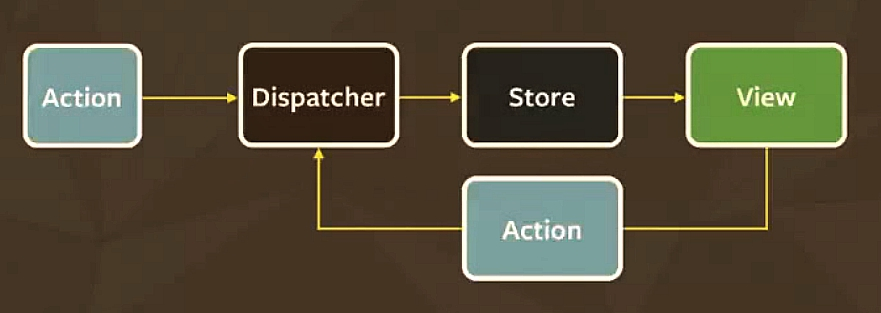
\includegraphics[scale=0.3]{n9.png}	
	\end{flushleft}	
	\textbf{Non è il pattern MVC}\\
	Flusso delle azioni: vengono generate dalla view, registrate presso un dispatcher, passate agli stores ecc...	
\end{frame}



